\documentclass[a4paper]{arrowhead}

\usepackage[yyyymmdd]{datetime}
\usepackage{etoolbox}
\usepackage[utf8]{inputenc}
\usepackage{multirow}

\renewcommand{\dateseparator}{-}

%% Special references
\newcommand{\fref}[1]{{\textcolor{ArrowheadBlue}{\hyperref[sec:functions:#1]{#1}}}}
\newcommand{\mref}[1]{{\textcolor{ArrowheadPurple}{\hyperref[sec:model:#1]{#1}}}}
\newcommand{\pdef}[1]{{\textcolor{ArrowheadGrey}{#1\label{sec:model:primitives:#1}\label{sec:model:primitives:#1s}\label{sec:model:primitives:#1es}}}}
\newcommand{\pref}[1]{{\textcolor{ArrowheadGrey}{\hyperref[sec:model:primitives:#1]{#1}}}}

\newrobustcmd\fsubsection[3]{
  \addtocounter{subsection}{1}
  \addcontentsline{toc}{subsection}{\protect\numberline{\thesubsection}function \textcolor{ArrowheadBlue}{#1}}
  \renewcommand*{\do}[1]{\rref{##1},\ }
  \subsection*{
    \thesubsection\quad
    function
    \textcolor{ArrowheadBlue}{#1}
    (\notblank{#2}{\mref{#2}}{})
    \notblank{#3}{: \mref{#3}}{}
  }
  \label{sec:functions:#1}
}
\newrobustcmd\msubsection[2]{
  \addtocounter{subsection}{1}
  \addcontentsline{toc}{subsection}{\protect\numberline{\thesubsection}#1 \textcolor{ArrowheadPurple}{#2}}
  \subsection*{\thesubsection\quad#1 \textcolor{ArrowheadPurple}{#2}}
  \label{sec:model:#2} \label{sec:model:#2s} \label{sec:model:#2es}
}
%%

\begin{document}

%% Arrowhead Document Properties
\ArrowheadTitle{EventPublish}
\ArrowheadServiceID{event-publish}
\ArrowheadType{Service Description}
\ArrowheadTypeShort{SD}
\ArrowheadVersion{4.3.0}
\ArrowheadDate{\today}
\ArrowheadAuthor{Szvetlin Tanyi}
\ArrowheadStatus{RELEASE}
\ArrowheadContact{szvetlin@aitia.ai}
\ArrowheadFooter{\href{www.arrowhead.eu}{www.arrowhead.eu}}
\ArrowheadSetup
%%

%% Front Page
\begin{center}
  \vspace*{1cm}
  \huge{\arrowtitle}

  \vspace*{0.2cm}
  \LARGE{\arrowtype}
  \vspace*{1cm}

  \Large{Service ID: \textit{"\arrowid"}}
  \vspace*{\fill}

  % Front Page Image
  %\includegraphics{figures/TODO}

  \vspace*{1cm}
  \vspace*{\fill}

  % Front Page Abstract
  \begin{abstract}
    This document describes a variant of the EventPublish service.
  \end{abstract}

  \vspace*{1cm}

  \scriptsize
  \begin{tabularx}{\textwidth}{l X}
    \raisebox{-0.5\height}{
\includegraphics[width=2cm]{figures/artemis_logo}} & {ARTEMIS Innovation Pilot Project: Arrowhead\newline
    THEME [SP1-JTI-ARTEMIS-2012-AIPP4 SP1-JTI-ARTEMIS-2012-AIPP6]\newline
    [Production and Energy System Automation Intelligent-Built environment and urban infrastructure for sustainable and friendly cities]}
  \end{tabularx}
  \vspace*{-0.2cm}
\end{center}
\newpage
%%

%% Table of Contents
\tableofcontents
\newpage
%%

\section{Overview}
\label{sec:overview}

This document describes the Event Publish Eclipse Arrowhead service, which enables event publishing.
Examples of this interaction is an event occurred at provider system and it wants to publish this event with some payload.

The rest of this document is organized as follows.
In Section \ref{sec:functions}, we describe the abstract message functions provided by the service.
In Section \ref{sec:model}, we end the document by presenting the data types used by the mentioned functions.

\newpage

\section{Service Interfaces}
\label{sec:functions}

This section lists the functions that must be exposed by the Event Publish service in alphabetical order.
In particular, each subsection names an abstract interface, an input type and an output type, in that order.
The input type is named inside parentheses, while the output type is preceded by a colon.
Input and output types are only denoted when accepted or returned, respectively, by the interface in question.

All abstract data types named in this section are defined in Section \ref{sec:model}.

\fsubsection{Event Publish}{PublishRequest}{}

This function is used to publish an event.

\newpage

\section{Information Model}
\label{sec:model}

\begin{figure}[t!]
  \centering 
  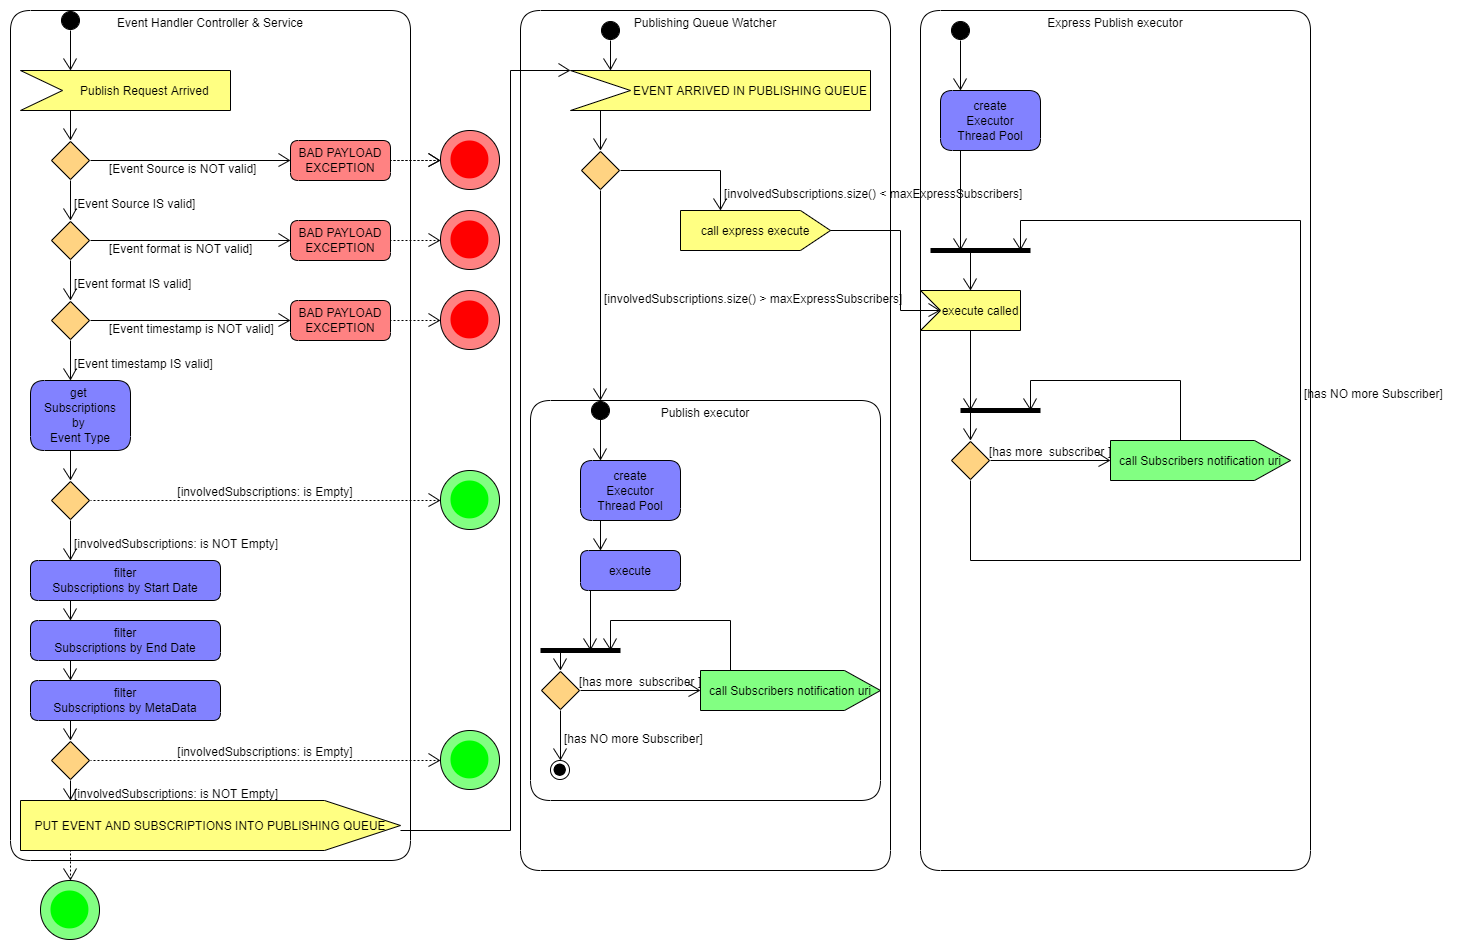
\includegraphics[width=0.8\textwidth]{figures/PublishEvent.png}
  \caption{Event Publish Activity Diagram. v4.3.0 only support HTTP/JSON/TLS.}
  \label{fig:EH_Publish}
\end{figure}

Here, all data objects that can be part of the EventPublish service calls are listed in alphabetic order.
Note that each subsection, which describes one type of object, begins with the \textit{struct} keyword, which is used to denote a collection of named fields, each with its own data type.
As a complement to the explicitly defined types in this section, there is also a list of implicit primitive types in Section \ref{sec:model:primitives}, which are used to represent things like hashes and identifiers.

\msubsection{struct}{PublishRequest}

This structure is used by a provider to broadcast its event.

\begin{table}[ht!]
\begin{tabularx}{\textwidth}{| p{5cm} | p{5cm} | X |} \hline
\rowcolor{gray!33} Object Field & Value Type      & Description \\ \hline
"eventType"  & \pref{String}    & Type of the event. \\ \hline
"metaData"   & \pref{Metadata}  & Metadata. \\ \hline
"payload"    & \pref{String}    & Event payload. \\ \hline
"source"     & \pref{System}    & Source system \\ \hline
"timestamp"  & \pref{DateTime}  & When the event occurred \\ \hline

\end{tabularx}
\end{table}

\subsection{Primitives}
\label{sec:model:primitives}

Types and structures mentioned throughout this document that are assumed to be available to implementations of this service.
The concrete interpretations of each of these types and structures must be provided by any IDD document claiming to implement this service.

\begin{table}[ht!]
\begin{tabularx}{\textwidth}{| p{3cm} | X |} \hline
\rowcolor{gray!33} Type & Description \\ \hline
\pdef{DateTime}        & A moment in time.  \\ \hline
\pdef{Metadata}        & Metadata \\ \hline 
\pdef{String}             & A string identifier that is intended to be both human and machine-readable. \\ \hline
\pdef{System}           & An \pref{Object} describing a system. \\ \hline
\end{tabularx}
\end{table}

\newpage

\bibliographystyle{IEEEtran}
%\bibliography{bibliography}

\newpage

\section{Revision History}
\subsection{Amendments}

\noindent\begin{tabularx}{\textwidth}{| p{1cm} | p{3cm} | p{2cm} | X | p{4cm} |} \hline
\rowcolor{gray!33} No. & Date & Version & Subject of Amendments & Author \\ \hline

1 & 2020-12-05 & 1.0.0 & & Tanyi Szvetlin \\ \hline

\end{tabularx}

\subsection{Quality Assurance}

\noindent\begin{tabularx}{\textwidth}{| p{1cm} | p{3cm} | p{2cm} | X |} \hline
\rowcolor{gray!33} No. & Date & Version & Approved by \\ \hline


1 &  &  & \\ \hline
 
\end{tabularx}

\end{document}